\documentclass[12pt,a4paper,oneside]{report}

% Add paths to look through
\makeatletter
\def\input@path{{Classes/}{preface/}{introduction/}{method/}{packing/}{dynamics/}{crystallisation/}{conclusion/}{appendix/}}
\makeatother


\usepackage{thesis}
\usepackage{preamble}

% Paths of figures
\graphicspath{{preface/figures/} {introduction/figures/}{dynamics/figures/}{packing/figures/}{crystallisation/figures/}}

% To include only some sections in the output, saves typesetting the entire thesis when working on a small section.
\includeonly{packing}

\begin{document}
\title{The Role of Molecular Shape on the Properties of the Condensed Phase:\\ A Simulation Study}
\author{Malcolm Ramsay}
\uni{The University of Sydney}
\dept{School of Chemistry}
\crest{\includegraphics[width=25mm]{USYD_logo}}
\principaladviser{Professor Peter Harrowell}
\coprincipaladvisor{Dr Asaph Widmer-Cooper}


\beforepreface

\prefacesection{Abstract}

\towrite{Abstract}

\prefacesection{Statement of Contribution}

\towrite{Contributions}

\contributionsignature

\prefacesection{Acknowledgements}

\towrite{Acknowledgements}

\prefacesection{Publications}

Work from Chapter 3 has been submitted for publication

\towrite{publication details}

\todototoc\listoftodos

\afterpreface




\chapter{Introduction}



Manipulating the formation of a condensed phase is a critical part of both nature and technology. From molluscs controlling crystal formation~\cite{de-yoreo:03}, to molecular glasses to increasing the solubility of drugs~\cite{hancock:00}, to plastics\tocite, silicon in photovoltaic cells\tocite, and many other materials that we rely on every day. As the devices we use become smaller the need to understand the processes that form them becomes more important. A complete theory of glass formation is still elusive and our ability to control crystal formation is far from what is available to nature. To better understand the formation of the solid phase, we need an understanding of the molecular rearrangements that take place as we move from a molecular liquid, through a supercooled liquid to either a glass or molecular crystal.

The goal of my project is to explore fundamental features of molecular shape; asymmetry and concavity, influence the properties of the various condensed phases; liquid, crystal, glass and supercooled-liquid. This requires the characterisation of a new set of molecular models for computer simulation. I will be addressing how the molecular orientation and translational motion couple during crystal growth, how the degree of concavity in the molecular shape determines the dynamics of rotations and translations in the low temperature liquid phase and, to find stable structures that determine the properties of crystals and glasses and how these structures are influenced by molecular shape.\tofix{This whole bit}


\section{Molecular Crystals}

The unit cell is the building block of a crystal, as such it is a useful tool to be able to describe the type of crystal. It is commonly used to describe metal salts, there is the \ce{CsCl} structure, or \ce{NaCl}, Zinc blende and many others. These are used because they are common materials characteristic of their unit cell structure, however the names do not directly inform us of the properties of the underlying unit cell. The simplest descriptor of the unit cell is the shape of the lattice system. There are 7 of these systems representing the different shapes that can be used to pack three dimensional space. Some of these lattice systems can then be combined with a lattice centering, an extra point or points on which a molecule is placed within the lattice. Taking the cubic lattice system as an example, there is the primitive (P) lattice centering where there are only lattice points on the corner of the unit cell which is the lattice of the primitive cubic packing of spheres. The second lattice centering is body centered (I) where there is an additional lattice point in the center of the lattice system resulting in the face centered cubic lattice. There is also the face lattice centering (F) where there is an additional lattice point on each face of the unit cell, for spheres this gives the densest known packing, the face centered cubic packing. The final lattice centering is the base (C) where there is an extra lattice point on one pair of opposing sides. This lattice centering is not present in the cubic lattice system. The combination of these lattice systems and lattice centerings gives the 14 \emph{Bravais lattices}~\figref{bravais}. 

\begin{figure}
    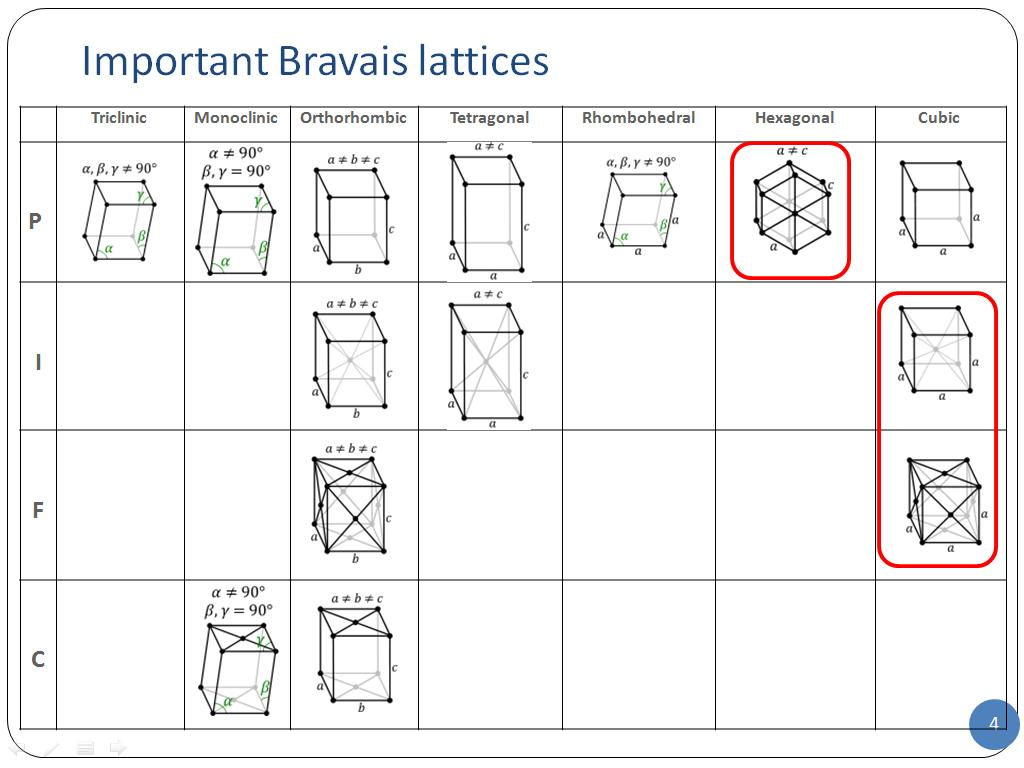
\includegraphics[width=\textwidth]{bravais_lattices}
    \caption{Modifying the seven lattice systems with lattice centerings gives the 14 Bravais lattices. TO LICENCE}
    \label{fig:bravais}
\end{figure}

While extensive, the Bravais lattices are not a complete description of the unit cell, especially in the case of molecules. There is no information on the relative orientation of molecules at each of the lattice points, the orientation of each molecule would have to be defined separately. There is a more complete description of the unit cell known as the \emph{space group}. The unit cell can be completely recreated from the space group, the unit cell parameters, and the position and orientation of a single molecule within the unit cell. Space groups are the combination of a set of symmetry operations and one of the Bravais lattices resulting in 219 space groups, 230 when including chiral copies. There are five symmetry operations that are important to space groups: reflection, rotation, improper rotation (a rotation combined with a mirror plane), screw axis (rotation and translation), and glide plane (reflection and translation)~\figref{symmetry ops}. This complete description of unit cells using space groups allows simple comparisons of crystal structures.


\begin{figure}
    \todofigure{Symmetry Operations}
    \caption{Diagram showing the symmetry operations}
    \label{fig:symmetry ops}
\end{figure}

When metallic crystals are grouped into their respective space groups there is a fairly even distribution amongst all the space groups~\figref{space dist}. Do the same with molecular crystals and there is a very different distribution, the $P2_{1/c}$ space group contains over a third of all molecular crystals~\tocite and the five most populous space groups contain \SI{75}{\percent} of all molecular crystals. To explain why molecules prefer these space groups over all the others we look to the simpler case of 2D. Using two dimensions has many benefits over a three dimensional system. Computations are far quicker in two dimensions, the complexity of the calculation is often to the power of the dimension, instead of dealing with $n^3$ calculations there are only $n^2$; a big difference when $n$ is large. The visualisation of a two dimensional system on a two dimensional interface such as a computer monitor or a piece of paper is also simpler, not having to deal with issues such as perspective. This makes visual identification of a pattern or property that incites Issac Asimov's famous ``that's funny'' response far more likely. Another benefit of working in 2D is that there are only 17 \emph{wallpaper groups}~\figref{wallpaper}, the 2D equivalent of space groups. Wallpaper groups are constructed in the same way as space groups and it is easier to identify the symmetry operations. In a similar manner to 3D we can group all the 2D molecular shapes that have been studied into their wallpaper groups~\figref{wallpaper dist}. In this case there are two wallpaper groups that contain the vast majority of molecules, the p2 and the p2gg wallpaper groups. As a general guideline for the packing of 2D molecules without central symmetry, Torquato and Jiao~\cite{torquato:12} suggest that the molecules will pair such that the pair will have an inversion center~\figref{molecule pair}. The only wallpaper groups that support pairs of molecules with this inversion center are the p2 and the p2gg, suggesting that the pairing of molecules has reasonable basis. This concept of an inversion center also applies to the 3D system, the $P2_{1/c}$ space group also has an inversion center and generally inversion centers are favoured~\cite{brock:94}.

\begin{figure}
    \todofigure{Distribution of metallic and molecular space groups}
    \caption{Showing the distribution of molecular crystals amongst the space groups}
    \label{fig:space dist}
\end{figure}

\begin{figure}
    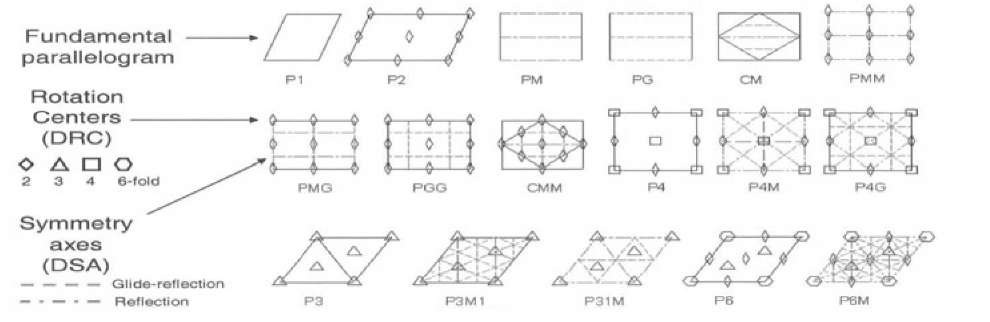
\includegraphics[width=\textwidth]{wallpaper_groups}
    \caption{Showing all the wallpaper groups and the symmetry operations that comprise them. TODO LICENCE}
    \label{fig:wallpaper}
\end{figure}

\begin{figure}
    \todofigure{Distribution amongst wallpaper groups}
    \caption{Distribution of 2D molecules amongst the 17 wallpaper groups}
    \label{fig:wallpaper dist}
\end{figure}

\begin{figure}
    \todofigure{Paired molecules}
    \caption{When molecules are non centrally symmetric they tend to pair creating an inversion center}
    \label{fig:molecule pair}
\end{figure}

The way that molecular crystals pack space is an important problem in simulating crystal structures. One of the methods used to find the optimal crystal structure is to model the molecule as an arrangement of hard spheres and find the arrangement of molecules that occupies the largest volume of space~\cite{kitaigorodskii:73}, also known as the \emph{packing fraction}. The simplest example of this is packing spheres, to which Kepler proposed that the hexagonal close packed structure was the most efficient in 1611~\cite{kepler:1611}. The hexagonal close packed structure has the same packing fraction as the face centered cubic structure despite being structurally distinct. While these structures have been considered the best possible packing of spheres in space for hundreds of years there has not been a mathematical proof until recently. In 2005 \textcite{hales:05} published a 400 page proof of this problem of which mathematicians were \SI{99}{\percent} certain was correct. Nearly 10 years later Hales {\em et al.}~\cite{hales:14} announced the completion of a project to completely satisfy the proof, using computers to check all possible configurations. 

\begin{figure}
    \todofigure{Close packed spheres}
    \caption{There are two structurally distinct closest packings of spheres, the hexagonal close packed structure and the cubic close packed structure}
    \label{fig:sphere packing}
\end{figure}

If finding a proof for the simplest of shapes was so difficult, how hard is it going to be to find closest packings for arbitrary shapes. While having a mathematical proof of the closest packed structure is nice, it is not necessary to perform useful chemistry, using the closest known packed structure is a reasonable alternative. Without the requirement for proof of correctness the problem of finding the closest known packing of arbitrary shapes becomes far simpler. The degrees of freedom of the particles can be considered a multidimensional space with the value at each point in space being the packing fraction~\figref{packing space}, finding the solution is now a case of finding the global minimum of this multidimensional function. Finding the global minimum of a function is a problem that appears in many fields, including computer science. As such there are a number of algorithms that can be used in an attempt to find the global minimum~\tocite. It should be noted that the only method that guarantees finding the global minimum is to evaluate packing fraction at every possible configuration. This is not computationally possible for any reasonably sized system, the number of points required scales exponentially with the number of molecules, quickly running into calculations that would take longer than the age of the universe. Many of these approximations use the concept of simulated annealing~\tocite. This is the process by which the configuration is given an amount of energy to move around the configuration space, moving out of a configuration that has a low packing fraction happens with a high probability, while moving out of a well where the packing fraction is high occurs with low probability. The probability of the configuration moving scales with the energy, as the energy is slowly reduced only the best configurations are sampled. If the energy is reduced slowly enough the global minimum is the final configuration, however there is no way to determine beforehand what slowly enough is. This concept comes from the process of glass formation which will be discussed in~\secref{} and many of the same concepts hold.

\begin{figure}
    \todofigure{Visualisation of packing space to search}
    \caption{}
    \label{fig:packing space}
\end{figure}

Much of the work that has been done in determining best packed structures has dealt with convex particles. These are fairly easy to pack efficiently. The shape with the worst packing efficiency of a centrally symmetric convex shape in 2D is the curved octahedron with a packing efficiency of 0.90~\tocite. While dealing with the packing of convex shapes is suitable for metallic crystal, when dealing with molecules concavities appear when holding two touching spheres in any orientation~\figref{concavity}.

\begin{figure}
    \todofigure{Overlapping spheres showing concavity}
    \caption{}
    \label{fig:concavity}
\end{figure}

\towrite{results of packing stuff}

Along with categorising the crystal structure the unit cell of a crystal structure is also responsible for many of the properties of the resulting material.

\towrite{Properties of solids, magnetic, conductivity, brittleness, piezoelectric}

\towrite{Link to liquids - Properties of the crystal degrade when transitioning to the liquid phase}

\section{Molecular Liquids}

The liquid phase is defined by its incompressibility and its ability to flow. There are two forces at play that define this behaviour. The ability to flow is comes from the energy of the particles, they have enough energy to move out of their local environments, but not enough to escape the attractive forces of the neighbouring particles as they flow around them. This attractive force is integral to the liquid phase, if the force is too short range or not present then the liquid phase does not exist~\tocite, only the solid and gas phases will form. When considering the process that occurs when a liquid flows, molecules must move away from their optimal position and around neighbouring molecules. If the attraction is too small at these larger distances there is nothing stopping the molecule flying off and becoming a gas. The other important force in a liquid is the repulsive force which is responsible for the structure of the liquid. A common measure of the structure of the liquid phase is the \emph{radial distribution function}~\figref{radial distribution} denoted $G(r)$. It can be calculated by
\begin{equation}
    G(r) = \text{maths}
\end{equation}
where stuff is defined. In essence it maps the probability of finding molecules at a distance $r$ from any particle, however unlike a probability the radial distribution function is normalised to $N-1$ where $N$ is the total number of particles in the system. It can also be expressed as the term that when multiplied by the density $\rho$ gives the local density around a particle. The radial distribution function gives a very clear distinction between between the crystal, and liquid and gas phases~\figref{radial distribution}. In the liquid phase phase we can see there is a region of excluded volume at small $r$, this is the result of the repulsive force, the apparent size of the molecule. Beyond the excluded region there is a sharp peak corresponding to the shell of nearest neighbours around the central molecule. It is the excluded region and short range ordering that results in the incompressibility, there is nowhere for the particles to move upon compression because of the repulsive force. The final part of the radial distribution function is the long range behaviour, for liquids there is no long range ordering, while for crystals there are peaks out to very large $r$. The radial distribution function is very useful when modelling systems where it is easy to calculate the distance between each particle, for experimental systems this is not possible. The usefulness of the radial distribution function is that is can be linked to a directly measurable quantity, the \emph{static structure factor} by a Fourier transform
\begin{equation}
    G(r) = \text{some function, structure factor}
\end{equation}
The static structure factor can be experimentally determined by taking the x-ray diffraction pattern of a sample providing the link between experimental and theoretical systems. Along with the structural differences between a liquid and a crystal there are also significant dynamical differences.

\begin{figure}
    \todofigure{Radial distribution functions}
    \caption{}
    \label{fig:radial distribution}
\end{figure}

Two common dynamic properties of a liquid are the viscosity and diffusion. The viscosity ($\eta$) of a liquid is a property of the bulk liquid measured in \si{\poise} or \emph{units of poise}. The viscosity is a temperature dependent quantity, following an Arrhenius curve
\begin{equation}
	\eta = \text{Arrhenius}
\end{equation}
where $T_0$ is the viscosity at a known temperature $T_0$, \kb is the Boltzman constant, and $E_a$ is the activation energy. In this case the activation energy can be considered the energy required to move past the nearest neighbours. The Arrhenius relation holds because this activation energy remains constant throughout the temperature range. The viscosities of some common liquids are shown in \tabref{} showing the range that viscosities take. The other dynamic property is diffusion, this is a property of individual molecules. Diffusion in liquids is described by \emph{Brownian motion}, first postulated by Einstein in 1911~\tocheck. The motion of particles is described by a differential equation 
\begin{equation}
	\text{Brownian motion}
\end{equation}
which is broken into two parts, a stochastic function ($A(t)$) responsible randomness of the motion as well as a term for the force a particle requires to move through the liquid, a similar concept to the activation energy. The stochastic nature of this differential equation requires that it be solved as an ensemble average, with the motion of any single particle being random solving for a particular particle results in a random solution. This ensemble averaged solution gives the result that at short times relative to $\zeta^{-1}$ the mean squared displacement (MSD) is dominated by ballistic motion from the local vibrations of particles. However looking to longer times we get a relation
\begin{equation}
	\text{Diffusion constant relation}
\end{equation}
where \tofix{define all terms}. This can be simplified by \towrite{define diffusion constant}


\towrite{Link diffusion constant and viscosity}

When dealing with molecules, along with the motion of the molecules the rotations of the molecules is also important. 
\towrite{rotational relaxations}



\section{Supercooled Liquids}

Supercooled liquids are an important part of forming the solid phase. At the melting point of a crystal \si{\Tm} both the liquid phase and the solid phase have the same free energy, there is no preferred state. However along with the energy of each phase there is also an energy penalty at the boundary of each phase, this means that for crystal formation to occur there has to be free energy gained by the formation of the crystal that offsets the penalty of the surface effects. The free energy of the crystal phase is only lower than the liquid phase when the liquid is supercooled. The free energy gained by the crystal phase scales with the supercooling, increasing the speed of crystal growth just requires reducing the temperature. Reducing the temperature will increase the growth rate of the crystal while the nucleation event is limiting the growth. As the temperature decreases the diffusion constant increases~\secref{}, this also means that the movements at the interface of the crystal to get molecules to align become slower, this is also well pronounced in the rotations of molecules. These two competing forces result in a temperature dependence on the rate of crystallisation that for some supercooling has a maximum rate of crystallisation~\figref{crys rate}.

\begin{figure}
    \todofigure{crystallisation as a function of temperature}
    \caption{}
    \label{fig:crys rate}
\end{figure}

If we are dealing with a system containing a constant number of particles, constant temperature and constant pressure, the standard conditions when working in a laboratory, the free energy that we are concerned with is the \emph{Gibbs free energy} ($G$). The change in free energy can be calculated using
\begin{equation}
    \Delta G = \Delta H - T\Delta S
\end{equation}
where $\Delta H$ is the change in enthalpy and $\Delta S$ is the change in entropy. The temperature dependence on the entropy is the reason that larger supercoolings promote nucleation. The entropy of the system is also a temperature dependent quantity which scales with the number of degrees of freedom. In a crystal molecules are far more constrained than in a liquid giving the temperature dependence of entropy a more gradual slope~\figref{entropy}. The result of this is that if the supercooled liquid can be kept in the liquid state there is a point at which the entropy of the liquid is below that of the crystal. Continuing this down to absolute zero the entropy will at worst track the slope of the crystal meaning there is a lower entropy state than the crystal at \SI{0}{\kelvin}. This is known as the Kauzmann paradox~\cite{kauzmann:48} and the temperature at which the entropy of the supercooled liquid is projected to cross that of the crystal is the Kauzmann temperature (\si{\Tk}). Another important temperature when dealing with supercooled liquids is the \emph{glass transition temperature} (\si{\Tg}), defined as the temperature at which the viscosity of the supercooled liquid reaches \SI{e13}{\poise}. One of the theories of glass formation~\cite{debenedetti:01} is that the glass transition is the system providing a solution to the paradox, undergoing dynamical arrest above \si{\Tk} reducing the number of degrees of freedom.

\begin{figure}
    \todofigure{entropy of liquid and crystal phase}
    \label{fig:entropy}
\end{figure}


When dealing with dynamics of supercooled liquids in most cases the viscosity observes Arrhenius behaviour just like a liquid. When approaching the glass transition temperature (\si{\Tg}) there are a number of supercooled liquids that display super-Arrhenius behaviour~\figref{angell} where there is a temperature dependence in the activation energy~\cite{angell:91}. Supercooled liquids that display this temperature dependence on the activation energy are known as \emph{fragile} liquids, they are interesting because they suggest that the glass transition temperature is not just an arbitrary concept but an inherent property of a material. The typical example of a fragile liquid is \emph{o}-terphenyl which has been widely studied~\cite{greet:67}. The liquids that keep the Arrhenius behaviour over the entire temperature range are known as \emph{strong} liquids, with the prototypical example being silica (\ce{SiO2}). The fragility ($m$) of a supercooled liquid can be given by the slope given in~\figref{angell},
\begin{equation}
    m = \text{stuff here}
\end{equation}
This gives a range of fragilities from silica, $m = 1$ to \emph{o}-terphenyl, $m = ??$~\tocheck with everything in between~\tabref{}. It is interesting to note that along with \emph{o}-terphenyl many of the fragile supercooled liquids are molecular, this feeds the hypothesis that glass forming ability is in some way related to shape, it can not be the only contributing factor but is a line of investigation to pursue.

\begin{figure}
    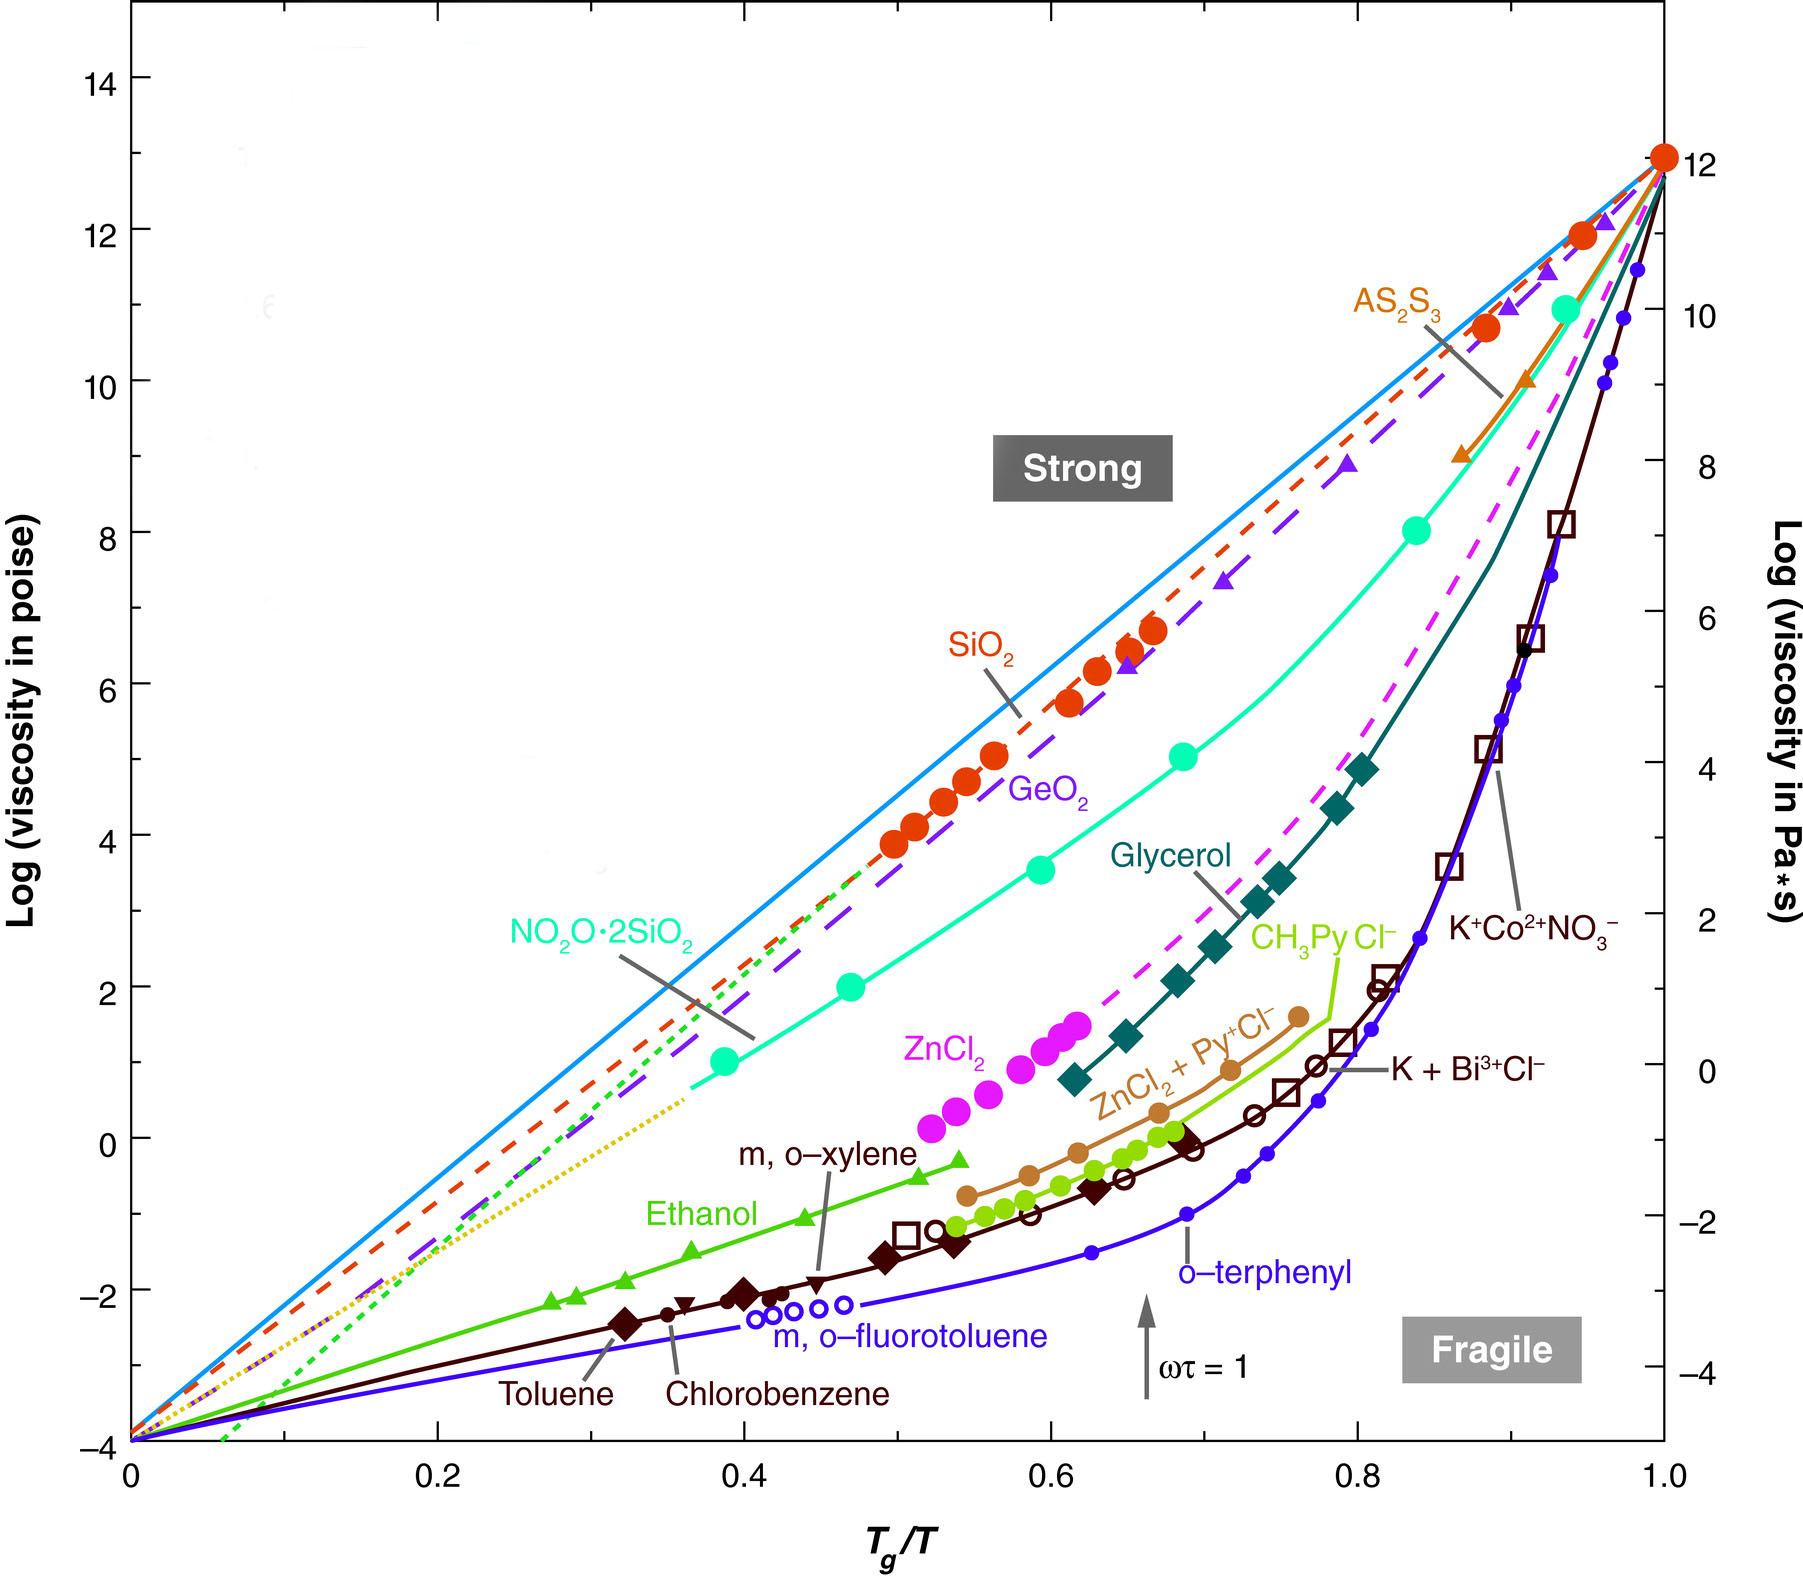
\includegraphics[width=\textwidth]{angell}
    \source{lubchenko:07}{Annual Reviews}
    \label{fig:angell}
\end{figure}

Along with the fragility of molecular glass formers, they are also interesting due to their rotational motion. In supercooled liquids below approximately \SI{1.2}{\Tg} there is a decoupling between rotational and translational diffusion~\tocite. It has been found that molecules translate faster than expected for their viscosity by as much as two orders of magnitude~\cite{debenedetti:01}. This results in molecules being able to move past each other but unable to rotate, limiting the range of states that can be sampled by the supercooled liquid. This is not the only decoupling present as close to \si{\Tg}, there is also a splitting of the relaxation frequency into two bands, the slow $\alpha$ relaxation and fast $\beta$ relaxation~\tocite. This decoupling in the relaxation can be explained by interpreting the supercooled liquid as a point on a multidimensional potential energy landscape, just like for the packing problem~\secref{}. Here the way that the supercooled liquid moves through the potential energy landscape is a function of the temperature. At high temperatures the liquid moves freely about the potential energy landscape, the energy of the molecules is often above any of the potential energy barriers. As the temperature gets lower the space of configurations available to the system gets smaller, there are potential energy barriers which only have a low probability of crossing. Close to the glass transition temperature the space of configurations is limited, there are many small local potential energy minima separated by larger energy minima. Moving between these larger minima requires a large number of rearrangements in the structure of the system, these movements correspond to the slow $\alpha$ relaxations~\figref{pe landscape}. The motion between the smaller energy minima are the $\beta$ relaxations resulting from small particle shifts.

\begin{figure}
    \todofigure{Potential energy landscape showing alpha a beta relaxations}
    \caption{}
    \label{fig:pe landscape}
\end{figure}

This topological view of the relaxation is consistent with a growing dynamic length scale, a property observed when approaching the glass transition~\cite{berthier:05}. At low temperatures the ability of the system to rearrange is very limited and requires coordinated rearrangement of a number of particles to move between each of the larger potential energy wells. Moving back into real space this growing dynamic length scale was first theorised when looking at dynamic heterogeneity~\cite{hurley:95} in model glass formers. These simulations showed areas of glasses that were highly mobile, where other regions were completely stationary. The mobile regions are those that are cooperatively moving as the liquid relaxes. As the supercooled liquid moves to lower temperatures larger regions have to move cooperatively, in the topological view this is where there is a barrier that is insurmountable in one direction, however by incorporating more particles and increasing the dimensionality the supercooled liquid can just move around the barrier~\figref{barrier dimensions}.

\begin{figure}
    \todofigure{Increasing dimensionality to go around barrier}
    \caption{In 2D space there is a barrier that is impassable, by including the 3rd dimension the traversal of the barrier is just a simple case of going around.}
    \label{fig:barrier dimensions}
\end{figure}

Taking these dynamic quantities to their limit, the glass transition temperature results in the formation of the glassy phase.


\section{Molecular Glasses}

The structure of a glass is indistinguishable from that of a liquid, the difference is that a glass has a viscosity of \SI{e13}{\poise}. Despite the liquid like structure, and urban legends~\tocite the glassy phase is most definitely solid, it would require a timescale of 100 million years for a glass with a viscosity at the glass transition to appreciably flow~\tocite. Much of the misunderstanding of the glassy phase is related to the lack of a first order phase transition~\tocite. None of the thermodynamic properties change upon transition, all the structural properties of the liquid phase apply to the glass phase, however the dynamics of the glass phase are far slower than any liquid. What does this mean for the glass phase? 

\towrite{Molecular glasses}
\begin{itemize}
    \item Jamming - 6 contacts
    \item Inherent structures
    \item out of thermodynamic equilibrium
\end{itemize}

Inherent structures are the structures generated when vibrations are removed, essentially structures at a temperature of \SI{0}{\kelvin}. These structures are interesting because it removes the complexity of vibrations, the structures are representative of the position of the atoms rather than their positions. In a way this is similar to taking x-ray diffraction patterns over timescales much longer than the vibration of the structure, the position observed is the average value, removing the noise generated by the vibrations. Removing vibrations is important for determining whether particles are within a cutoff to determine whether they are neighbouring, the vibrations can be easily large enough to push molecules inside or outside this cutoff producing noisy results. By taking a number of inherent structures at various temperatures~\figref{inherent structures} the effect that the temperature the inherent structure is equilibrated is easily observed. This means that any glassy state is dependent on its temperature history, glasses cooled quickly have different properties to those cooled slowly, a technique used for hundreds of years by glass blowers to produce more durable glass\tocite.

\begin{figure}
    \begin{centering}
    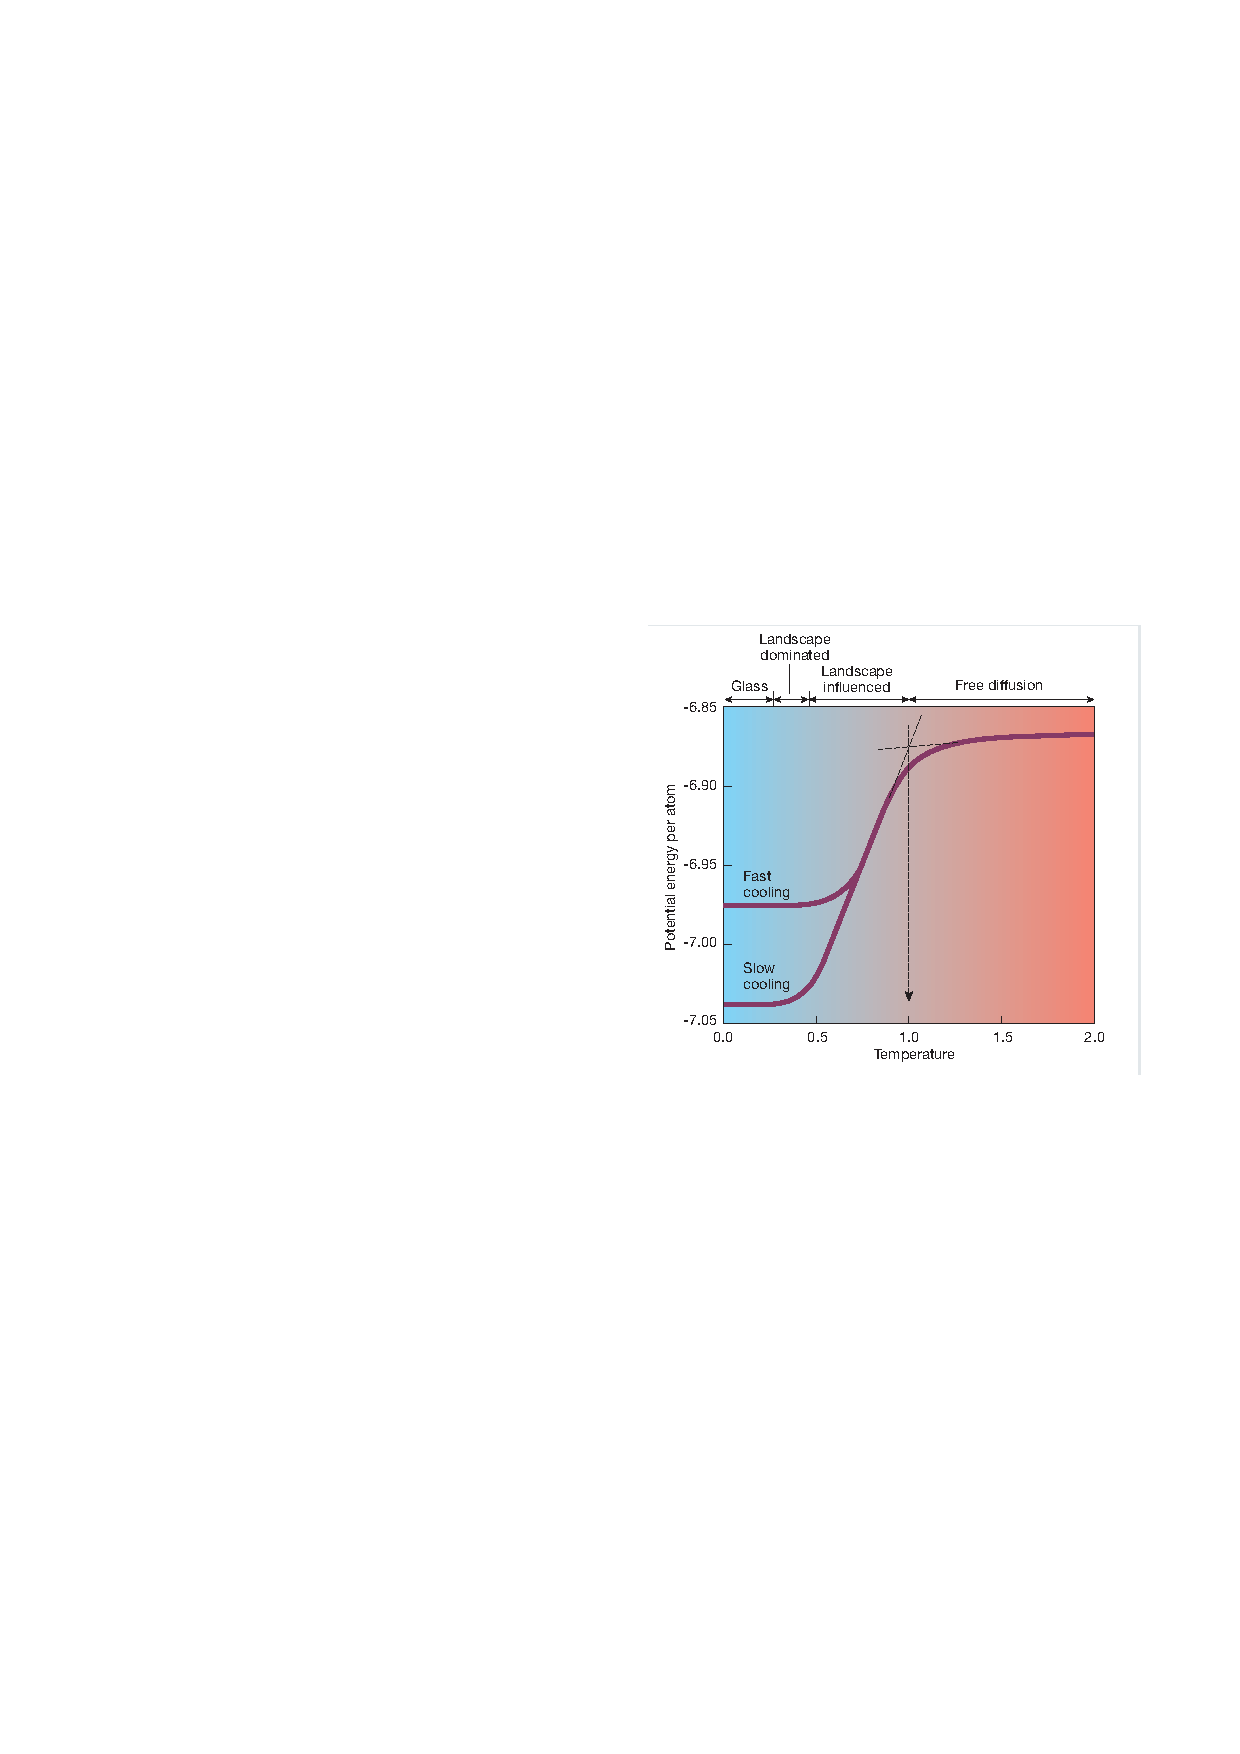
\includegraphics[width=0.5\linewidth]{inherent_structures}
    \caption{The mean inherent structure energy per particle of a binary Lennard-Jones mixture as a function of the temperature of the equilibrated liquid from which the inherent structures were generated. At high temperature the liquid can sample the entire energy landscape where most of the energy minima are shallow giving high energy inherent structures. At low temperatures many of the energy minima are inaccessible, the activation energy required to reach them exceeds the energy of the system. In the case of the fast cooling the system is stuck with an energy barrier between the states it can occupy and the lower energy states being occupied by the slow cooling.}
    \source{debenedetti:01}{Nature Publishing Group}
    \label{fig:inherent structures}
\end{centering}
\end{figure}

The algorithm commonly used to find the inherent structure is conjugate gradients\tocite. This is another algorithm focused on finding minima on a multidimensional landscape, $F(\vect x)$~\cite{shewchuk:94,hestenes:52}. In this case conjugate gradients is an iterative algorithm that will find the closest local minima in a small number of steps. The conjugate gradient algorithm is most simply explained as as extension of another iterative algorithm, steepest descent. The naming of the steepest descent algorithm is very self descriptive, a step of size $\gamma$ is taken in the direction of the steepest descent. Each step is given by
\begin{equation}
    \vect r_{i+1} = \vect r_i - \gamma \nabla F(\vect r_i)
\end{equation}
where $\vect r_i$ is the approximation to the minimum at step $i$ and
\begin{equation}
    \nabla = \left (\pddiff{}{x_1}, \pddiff{}{x_2},\cdots,\pddiff{}{x_n} \right )
\end{equation}
Steepest descent is limited in that it will often zig-zag slowly towards the minimum, requiring a large number of steps. The conjugate gradient method takes into account the direction of the previous step, with the new step being a linear combination of the previous step and the steepest descent at the current point
\begin{align}
    \vect r_{i+1} &= \vect r_{i} - \Delta \vect r_i \\
     \Delta \vect r_{i} &= \alpha( \nabla F(\vect r_i) + \beta \Delta \vect r_{i-1})
\end{align}
with constants $\alpha$ and $\beta$ which in practice are calculated each step for fastest convergence. Note that it is not possible to take a first step with the conjugate gradient algorithm, the direction of the previous step is needed. In practical applications of the conjugate gradient algorithm the initial step is taken using the steepest descent algorithm, with the remaining steps using conjugate gradient. Each step of the conjugate gradient algorithm requires more calculation than a step with the steepest descent algorithm, the improvement from using conjugate gradient comes from reducing the number of steps required~\cite{knyazev:08}.



\chapter{Method}

\section{Molecules}

The potential that I have chosen to use is a modified Lennard-Jones potential. This is a potential commonly used in molecular dynamics systems due to its simplicity to calculate. It is also the potential used by most studies on glass forming binary mixtures~\tocite. The potential takes the form
\begin{equation}
    V_{LJ}(r) = 4\epsilon\left [ \left (\frac{\sigma}{r}\right )^{12} -\left ( \frac{\sigma}{r} \right )^6 \right]
\end{equation}
where $r$ is the separation of two centers and, $\epsilon$ and $\sigma$ are parameters describing the strength and the size of the potential respectively. The computational simplicity comes from the 6th power function which is easy to compute, and the 12th power term is the square of the 6th power term. In the default form the potential for each particle acts on all other particles, despite most of these interactions being negligible. To account for this the potential is commonly modified to have a cutoff at some value of the potential; we chose a cutoff of $2.5\sigma$. The final modification to the potential is to retain the continuity of the original function, this involves subtracting the value at the cutoff giving a function of the form
\begin{equation}
    V_{mod}(r) = \begin{cases}
        \quad V_{LJ}(r) - V_{LJ}(2.5\sigma) & \text{if} r < 2.5\sigma \\
        \quad 0  &\text{if} r >= 2.5\sigma
    \end{cases}
\end{equation}
These particles were then constructed into molecules.

There were two types of molecule that we study in this thesis, Snowmen~\figref{snowman} and Trimers~\figref{trimer}. The Snowman molecule is constructed from two particles, a large and a small particle. The large particle has a radius 1, the size of the small particle $r$ is then a ratio to the size of the large particle. The only other variable in the Snowman particle is the distance $d$ between the centers of the two particles. The Trimer molecule is similar to the Snowman molecule, it also has a large particle of radius $1$, the difference is that there are two small particles of radius $r$ at distance $d$ subtended by an angle $\theta$.

\begin{figure}
    \begin{subfigure}{0.5\textwidth}
        \centering
        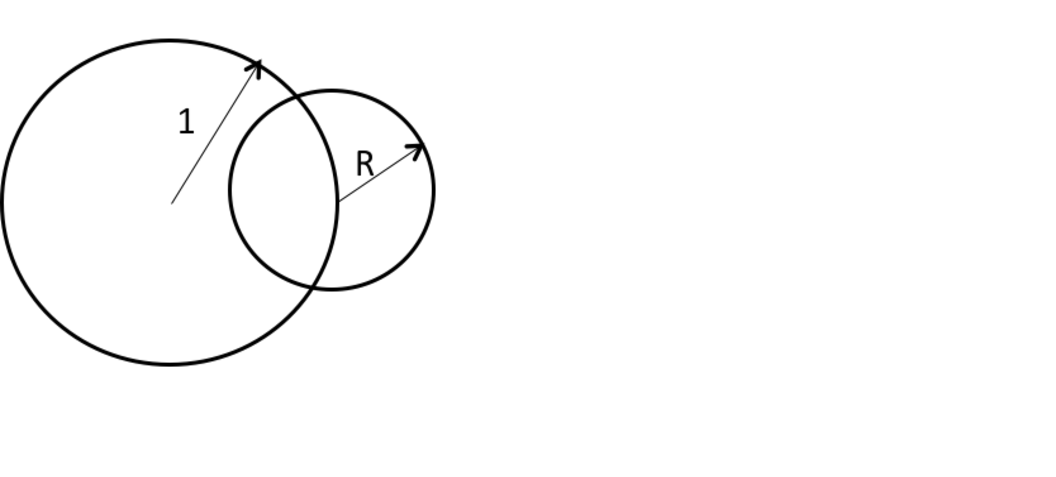
\includegraphics[width=\linewidth]{Snowman}
        \caption{Construction of Snowman molecules}
        \label{fig:snowman}
    \end{subfigure}
    \begin{subfigure}{0.5\textwidth}
        \centering
        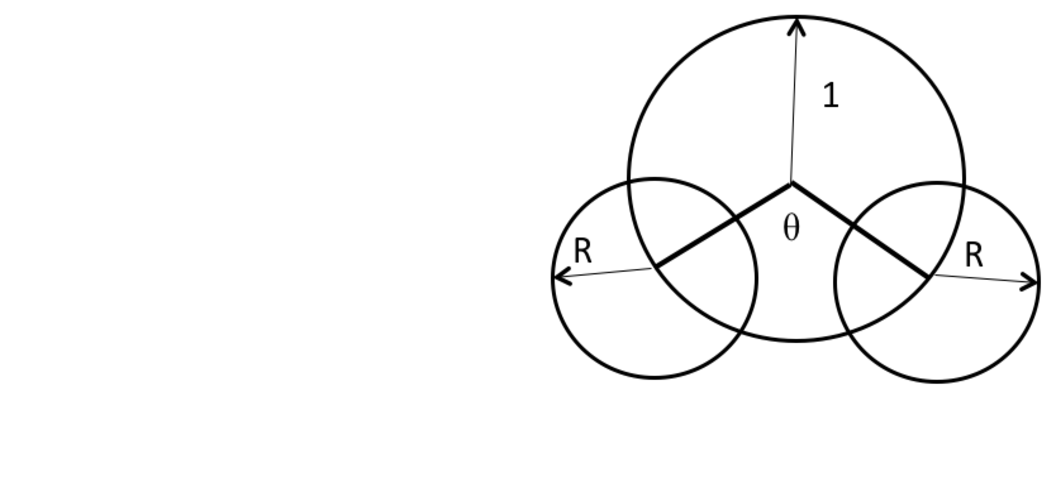
\includegraphics[width=\linewidth]{Trimer}
        \caption{Construction of Trimer molecules}
        \label{fig:trimer}
    \end{subfigure}
    \caption{Construction of the molecules used in this thesis}
    \label{fig:construction}
\end{figure}

The particles of each molecule are implemented as modified Lennard-Jones particles with $\epsilon = 1$ and $\sigma = 2r$. Interactions between combinations of particles are given by the average $r$. The bond lengths and angles use a harmonic potential with a spring constant $k=5000$, more than three orders of magnitude greater than the bonded interactions. This large spring constant is to keep the arrangement of the particles as close as possible to that of a rigid molecule.

\section{Molecular Dynamics}

The simulations in this thesis are performed using molecular dynamics, the positions of molecules are stepped through time by solving Newton's equations at each step. The software used to perform the molecular dynamics is Lammps~\tocite, an open source program designed to efficiently perform large scale molecular dynamics simulations. An integral part of the optimisation achieved by Lammps is the spatial decomposition of particles amongst the available processors, allowing for efficient use use of a large number of processors~\tocite. Spatial decomposition is a technique that divides the simulation area into a grid equal to the number of processors. Each processor is then assigned an area of the grid for which it is responsible for computing. The processors are also assigned a set of \emph{ghost particles}, particles which are outside of the region the processor is responsible for computing but are close enough to be applying a force to particles in that region. The use of ghost atoms reduces the amount of communication between processors, at each step the only communication required is the updated positions of the ghost atoms. The reduction in communication is important for efficiency as it is the major speed bottleneck in alternative methods.

Lammps implements the modified Lennard-Jones potential and also the associated reduced units.
\towrite{reduced units}

The thermodynamic ensemble for the simulation is the NPT ensemble, with a constant number of particles (N), constant pressure (P) and constant temperature (T). The constant number of particles is achieved by not adding or removing any particles from the simulation, the pressure and temperature are kept constant by a Noose-Hoover thermostat\tocheck.
\towrite{Thermostat and barostat}


\section{Specific Implementations}

\subsection{Packing}

The initial configuration for the random packings is a grid of molecules in a random orientation with a distance between them larger such that they are unable to contact each other. From this state the molecules are allowed to compress and equilibrate at a temperature $T=5$, well above the melting point. The configuration was then equilibrated at a series of lower temperatures with a quenched configuration taken at each temperature.

\subsection{Dynamics}

The initial state of these runs was the same as for the packing, however the series of temperatures was finer. The other difference is that the system was equilibrated at each temperature, before a production run, from which data as collected was performed. As the temperature gets lower the timescale of the dynamical phenomenon gets slower, the length of the production run was longer for lower temperatures.

\subsection{Crystal Structures}

\begin{itemize}
    \item Isopointal algorithm
    \item starting from Toby's structures
    \item Converting to large unit cell, squaring the edges
    \item equilibration at low T
    \item Rahman-Parinello
\end{itemize}

\subsection{Interface Kinetics}

\begin{itemize}
    \item Start with crystal
    \item Melt half holding other half in place
    \item equilibrate at temperature
    \item Production run
\end{itemize}

\section{Minimisation Algorithms}

The algorithm commonly used to find the inherent structure is conjugate gradients\tocite. This is another algorithm focused on finding minima on a multidimensional landscape, $F(\vect x)$~\cite{shewchuk:94,hestenes:52}. In this case conjugate gradients is an iterative algorithm that will find the closest local minima in a small number of steps. The conjugate gradient algorithm is most simply explained as as extension of another iterative algorithm, steepest descent. The naming of the steepest descent algorithm is very self descriptive, a step of size $\gamma$ is taken in the direction of the steepest descent. Each step is given by
\begin{equation}
    \vect r_{i+1} = \vect r_i - \gamma \nabla F(\vect r_i)
\end{equation}
where $\vect r_i$ is the approximation to the minimum at step $i$ and
\begin{equation}
    \nabla = \left (\pddiff{}{x_1}, \pddiff{}{x_2},\cdots,\pddiff{}{x_n} \right )
\end{equation}
Steepest descent is limited in that it will often zig-zag slowly towards the minimum, requiring a large number of steps. The conjugate gradient method takes into account the direction of the previous step, with the new step being a linear combination of the previous step and the steepest descent at the current point
\begin{align}
    \vect r_{i+1} &= \vect r_{i} - \Delta \vect r_i \\
     \Delta \vect r_{i} &= \alpha( \nabla F(\vect r_i) + \beta \Delta \vect r_{i-1})
\end{align}
with constants $\alpha$ and $\beta$ which in practice are calculated each step for fastest convergence. Note that it is not possible to take a first step with the conjugate gradient algorithm, the direction of the previous step is needed. In practical applications of the conjugate gradient algorithm the initial step is taken using the steepest descent algorithm, with the remaining steps using conjugate gradient. Each step of the conjugate gradient algorithm requires more calculation than a step with the steepest descent algorithm, the improvement from using conjugate gradient comes from reducing the number of steps required~\cite{knyazev:08}.

Both the steepest descent and the conjugate gradient methods are good at finding the local minimum. Often more important than local minima are the global minima, where other techniques are required. One case where finding the global minima is important is the formation of a crystal from a liquid phase. This is one of the common techniques, known in computer science as simulated annealing~\tocite, the idea is that you start at a high temperature and slowly reduce the temperature. If the reduction in temperature is slow enough the final state will be the global minimum of the function, otherwise it will be a local minima. This is exactly the process that is being investigated in this thesis using molecular dynamics to sample the possible space of the function describing the degrees of freedom of all the molecules with the state of the function given by the total energy of the molecules. Here the aim is to arrange the molecules in the lowest energy configuration, the crystal state. In some cases, like a single component disc liquid will easily crystallise~\tocite, other cases like certain binary disc mixtures~\tocite are highly resistant to crystallisation. In these cases there are other methods to find the lowest energy state.

Molecular dynamics simulations typically have a large number of particles to give a reasonable approximation of real world phenomena and to remove the effects of particles interacting with themselves through the periodic boundary conditions. These requirements are not always the case, by exploiting the symmetry of a space group and \emph{isopointal sets} the dimensionality and search space can be dramatically reduced~\cite{hudson:10}. An isopointal set is a space group and a minimal set of symetrically distinct sites, with the rest of the molecules in the unit cell generated by application of the symmetry operations. These minimal set of sites are known an \emph{Wyckoff} sites~\cite{gelato:87,bergerhoff:99}. These simplifications reduce the dimensionality of the problem significantly, each space group has a small set of possible Wyckoff sites, each with only a few optimisation parameters which can be optimised using \emph{Monte Carlo} simulated annealing.

The basis of \emph{Monte Carlo} methods is that the space of interest is traversed stochastically. It is used in a number of applications, the simplest application of this method is to approximate the area of a region in space. This can be done by taking an easy to calculate enclosing area, like a square, and an unknown area defined by some inequalities and generating a series of points in the larger area~\figref{monte carlo pi}. The fraction of points in the unknown area is an approximation of the relative size of the area. We can also consider this process as an accept/reject criterion, accept if in the area of interest, reject if not. In this case the percentage accepted is important. In simulated annealing this accept/reject criterion is related to the energy of the state, a high energy state is less likely to be accepted than a low energy state. As the temperature is reduced the region of acceptance shrinks along with the size of the jumps between configurations, with the final configuration ideally being the lowest energy configuration.

\begin{figure}
    \centering
    \animategraphics[loop,autoplay,width=0.5\linewidth]{3}{Pi-}{0}{9}
    \caption[Approximating $\pi$ using the monte carlo method]{Approximating $\pi$ using the Monte Carlo method using the ratio of points falling in each area. Increasing the number of points reduces the error in the result.}
    \source[\ccby]{montecarlopi}
    \label{fig:monte carlo pi}
\end{figure}




\chapter{Packing shapes on a Plane}

Shapes studying:
\begin{itemize}
    \item Shape - Snowman, Trimer
    \item Radius - 0.5 0.6 0.7 0.8 0.9 1.0
    \item Distance - 1.0 1+r
    \item Theta - 120, 180
\end{itemize}

Data gathered for each shape
\begin{itemize}
    \item High temp quench - T = 5.0
    \item Low temp quench - T = 0.5
    \item Optimal packing, structure from Toby, perform MD equil
\end{itemize}

Analysis
\begin{itemize}
    \item Configuration image
    \item Contact numbers ($f_6$)
    \item Radial distribution function ($g(r)$)
    \item Structure function ($s(q)$)
    \item Hexatic ordering 
\end{itemize}

Important figures
\begin{itemize}
    \item $f_6$, $s(q)$, hexatic function of radius
    \item Packing fraction comparison
    \item Comparison of high and low temp quench
\end{itemize}

\section{Packing Dimers}

It is widely documented that shape plays an important role in crystal packing, with small changes to the shape dramatically affecting the crystal structure. Amorphous packing however is an unstructured arrangement, small changes would just get averaged over the system.


I have studied how a number of small modifications to the shape of a molecule affects the amorphous packings. The amorphous packings are inherent structures taken from a liquid or glassy phase. The first of these is the effect of the relative sizes of the two discs. There are a number of binary disc mixtures that are glass forming~\tocite, the two sizes of discs incapable of packing better than individually. There are also a number of binary disc packings that provide optimal space coverage~\tocite, the small particles perfectly filling the gaps left by the large particles. When the two discs ($r_1 = 1, r_2 = r$) are held fixed at a distance of $1+r$ the packing is conceptually similar to a binary disc mixture however there is the extra constraint that the distance and orientation remains fixed. \textfigref{fix d var r} shows how the packing fraction compares to the optimal packing fraction, the optimal packings were found by Toby Hudson~\tocite and equilibrated using the same potential as the amorphous systems\toref. At $r = 1$ both the amorphous and the optimal crystal packing have the same packing fraction, looking at their configurations~\figref{config:d2r1} the individual particles pack as though they are just discs, the packing efficiency of individual particles is the same, however the rotational orientation of the molecules in the crystal structure is ordered, while the amorphous structure has the molecules randomly arranged in the 6 possible orientations\tocheck. This means the packing is not strictly amorphous.

\begin{figure}
    \todofigure{r = 0.5 - 1.0, d = 1+r vs packing fraction, compare to optimal}
    \caption{The packing efficiencies of amorphous snowmen compared to their optimal packing fraction.}
    \label{fig:fix d var r}
\end{figure}

\begin{figure}
    \todofigure{configuration of d=1 r=2 for both amorphous and crystal showing alignment of the molecules}
    \label{fig:config:d1r2}
    \caption{Both the amorphous and the crystal structure pack in the same way with only the orientations of particles differing between them}
\end{figure}

Another special crystal structure is where $d=1.637556$, this is one of the optimal binary packings~\figref{crys:d=1.637556}. Unlike where $d=2$ the packing fraction of this amorphous configuration is far lower than the crystal structure. This is interesting as both crystal structures are from the p2 or p2gg space groups, however the $d=2$ structure is easier to form than the $d=1.637556$.

\begin{figure}
    \todofigure{Structure of d=1.637556 snowman}
    \caption{Optimal packing of binary discs, small disc is 0.637556 times the size of the large disc.}
    \label{crys:d=1.637556}
\end{figure}

At smaller radii 
\towrite{what the smaller radii do, how they compare to the crystal packing}

The case where the two particles are at a distance of $1+r$ is an extreme case, molecules tend to have overlapping spheres, the overlap responsible for the bonding between them. As a result of this it makes sense to investigate the effect of distance on the amorphous packing. In \textfigref{var d fix r} shows how the packing fraction changes as a function of the distance where the radius of both particles is the same. There is a significant increase in the packing fraction as the radius decreases, this is as a result of the overlap of the particles filling more space. Despite this increase in the packing fraction the packing becomes amorphous as the distance decreases, then increasing again as the distance goes to 0. Rather than looking at every configuration and we need an order parameter to quantify the amount of order within the system.

\begin{figure}
    \todofigure{plot of d vs packing fraction for r = 1}
    \label{fig:var d fix r}
    \caption{Some words}
\end{figure}

\section{Order parameters}

There are many order parameters suitable for different types of systems, some more suitable than others.
\begin{itemize}
    \item Circle order (number of neighbours for d=1.637556)
    \item Packing fraction
    \item structure factor
    \item 6 fold order
    \item g(r)
    \item short range order
    \item orientational order
\end{itemize}

\begin{itemize}
    \item The 6 fold order parameter is most suitable for degree of crystallinity.
    \item g(r) for d=1 snowman

\towrite{fill out $\uparrow$}

\begin{figure}
    \begin{subfigure}{0.5\textwidth}
        \todofigure{Various order parameters for crystal and amorphous as a function of r}
        \caption{Order parameters for radii}
    \end{subfigure}
    \begin{subfigure}{0.5\textwidth}
        \todofigure{Various order parameters for crystal and amorphous as a function of d}
    \end{subfigure}
\end{figure}

\section{Packing Trimers}
\label{packing trimers}

There is another simple property that has the potential to have an effect on the amorphous structures, angle. To study angle we need to move from two particles to three.

\section{Shapes of Interest}
\label{shapes of interest}

The range of shapes, even simple ones is huge with a wide range of behaviour. It is not feasible to study this entire range of shapes in detail, the list of shapes need to be narrowed down to a range that is both interesting and representative of the wider spectrum of shapes.

\towrite{I chose d=1.637556 snowmen, here's why}



\chapter{Liquid Dynamics}

Molecules (<shape>-<radius>-<distance>-<theta>)
\begin{itemize}
    \item Snowman-0.637556-1.0
    \item Snowman-0.637556-1.637556
    \item Trimer-0.637556-1.0-120
\end{itemize}


Data
\begin{itemize}
    \item Snowman-0.637556-1.0
        \begin{itemize}
            \item T = 
        \end{itemize}
    \item Snowman-0.637556-1.637556
        \begin{itemize}
            \item T = 
        \end{itemize}
    \item Trimer-0.637556-1.0-120
        \begin{itemize}
            \item T = 
        \end{itemize}
\end{itemize}


Analysis
\begin{itemize}
    \item MSD
    \item Diffusion Constant
    \item Rotational relaxation (R1, R2)
    \item Rotational relaxation time (t1, t2)
    \item Structure function (f)
    \item Structural relaxation time (ts)
    \item Order parameter - neighbouring small and large particles
    \item Hexatic ordering
\end{itemize}

Key Plots
\begin{itemize}
    \item MSD for all T
    \item Rotations for all T
    \item Relaxation times function of 1/T
    \item Comparing d=1 to d=1+r
        \begin{itemize}
            \item Diffusion constant
            \item Rotational relaxations
            \item Structure functions
        \end{itemize}
\end{itemize}


\section{Characterisation}

The dynamics of a molecular system is characterised by two main elements, the diffusion of the particles through the liquid and the rotational motion of those particles. Understanding these properties of the liquid provide the basis for further study giving estimates of the timescales that events are likely to occur at. It also provides important information about the range of temperatures at which the particular system can be studied. The molecules that we have chosen for study are shown in \textfigref{shapes}, these molecules were chosen to be representative of the range of samples and also with the possibility of showing interesting behaviour as discussed in \textsecref{shapes of interest.

\begin{figure}
    \todofigure{Shapes being studied for dynamics}
    \caption{The shapes being studied in this chapter}
\end{figure}



 \section{d=1+r}

\section{Oh hey they are different}


\chapter{Crystallisation}

In this chapter we apply the concepts of both dynamics and structure to investigate the dynamics of ordering. The vibrations of the molecules make the analysis of dynamical structure more difficult with far more noise as a result of the vibrations.

\section{Melting Points}


\begin{table}
    \centering
    \begin{tabular}{ | c  l | S S S S S |}
        \hline
        Molecule & Crystal & {Melting Point} & {$H_\text{amorphous}$} & {$H_\text{crys}$} & {$\Delta H$} & {$\Delta S$} \\ \hline
        \done & p2mg & 0.80 & & & & \\
        \dcon & p2   & 1.90 & & & & \\
        \tri  & p2   & 1.40 & & & & \\
        \hline
    \end{tabular}
\end{table}


\section{Crystallisation Dynamics}


\subsection{Two Phase Systems}

To get around the issues of waiting for a nucleation event to occur to see the growth of a crystal, we can create a two phase system in which the liquid-crystal boundary is already present. This can then be used to observe the growth of the crystal phase on this surface. Using these two phase configurations as the starting point we see crystallisation of the \done molecule~\figref{done crys}. It is interesting to note that the preferred crystal growth direction is at a \SI{45}{\degree} angle to the crystal boundary. Along with the crystal growth at the existing crystal interface there is also the nucleation of large crystals from the liquid, nucleation may be a fairly common event for the \done molecule.

\begin{figure}
    \begin{subfigure}{\textwidth}
        \includegraphics[width=\textwidth]{{{Snowman-0.75-0.637556-1.0-p2mg-1-frame-0000000000}}}
        \caption{Initial configuration of the two phase system for the \done crystal.}
    \end{subfigure}
    \begin{subfigure}{\textwidth}
        \includegraphics[width=\textwidth]{{{Snowman-0.75-0.637556-1.0-p2mg-1-frame-0320000000}}}
        \caption{Final configuration of the two phase system of the \done crystal.}
    \end{subfigure}
    \caption{A two phase system of the \done molecule with the favoured p2mg crystal in the center. The temperature is held at 0.75. Molecules considered as crystalline are coloured according to their orientation such that molecules that are antiparallel will have the same colour, non-crystalline molecules are grey. This system promotes growth at the boundary of the crystal as seen by the expanding region of teal colour.}
    \label{fig:done crys}
\end{figure}

The two phase analysis can also be performed on the \dcon system~\figref{dcon crys}. The order parameter we are using for the \dcon system appears to be less robust than for the \dcon system, \textfigref{dcon crys} shows many false negatives within the crystal system, while there are also more false positives, individual particles deemed as crystalline. However despite the issues with the order parameter we are able to see a growth in crystallisation~\figref{dcon crys fine}, the regions where the ordered phase is lacking orientational order are regions of growth of the crystal. These orientationally disordered regions have to have come from the liquid phase as the crystal phase has all molecules in an antiparallel orientational order. Also like the \sone molecule we observe the spontaneous nucleation of ordered regions.

\begin{figure}
    \begin{subfigure}{\textwidth}
        \includegraphics[width=\textwidth]{{{Snowman-1.60-0.637556-1.637556-p2-1-frame-0000000000}}}
        \caption{Initial configuration of the two phase system of the \dcon molecule.}
        \label{fig:dcon crys init}
    \end{subfigure}
    \begin{subfigure}{\textwidth}
        \includegraphics[width=\textwidth]{{{Snowman-1.60-0.637556-1.637556-p2-1-frame-0320000000}}}
        \caption{Final configuration of the two phase system of the \dcon molecule.}
        \label{fig:dcon crys fine}
    \end{subfigure}
    \caption{Two phase system of the \dcon molecule with the favoured p2 crystal in the center. The temperature of this system is held at 1.60. Molecules considered ordered are coloured according to their orientation while molecule slacking order are grey. Growth of the crystal can be seen as coloured regions lacking the orientational order of the central crystalline region.}
    \label{fig:dcon crys}
\end{figure}

Unlike the \done and \dcon molecules the \tri molecules does not show crystallisation in the two phase system~\figref{tri crys}. The trimer shows small changes on the surface of the crystal between the initial~\figref{tri crys init} and the final~\figref{tri crys fine} configurations however these are more like what would occur at equilibrium, a rearrangement of the surface rather than growth, despite being below the melting point of the crystal phase. One explanation for this behaviour is the timescale that we are looking at is short compared to the rate of crystal growth.

\begin{figure}
    \begin{subfigure}{\textwidth}
        \includegraphics[width=\textwidth]{{{Trimer-1.30-0.637556-1.00-120-p2-1-frame-0000000000}}}
        \caption{Initial configuration of the two phase system of the \tri molecule.}
        \label{fig:tri crys init}
    \end{subfigure}
    \begin{subfigure}{\textwidth}
        \includegraphics[width=\textwidth]{{{Trimer-1.30-0.637556-1.00-120-p2-1-frame-0320000000}}}
        \caption{Final configuration of the two phase system of the \tri molecule.}
        \label{fig:tri crys fine}
    \end{subfigure}
    \caption{Two phase system of the \tri molecule with the favoured p2 crystal in the central region. The temperature of this system is held at 1.30. Molecules considered ordered are coloured according to their orientation such that molecules that are antiparallel are coloured the same while non-crystalline regions are grey. Despite being below the melting point of the crystal there is no significant net growth of the crystal phase.}
    \label{fig:tri crys}
\end{figure}

\subsection{Spontaneous Nucleation}

We have seen spontaneous nucleation from both the \done and \dcon molecules in the two phase system. We want to be able to see this nucleation from a random starting phase, to show that this is not just a remnant of order from the crystal the liquid phase was melted from. To see this nucleation we had to run simulations far longer than the simulations for dynamics.

The \done molecule shows significant regions of crystallinity~\figref{done nuc}. The configuration is dominated by a number of peach coloured crystals, the dominance of this orientation can be explained by examining the bottom right corner, between above the crystal there are layers of molecules with a more complex ordered structure, this structure forms most of the links between the peach crystal regions keeping them aligned. The other interesting feature of the crystal structure is the boundary between the lavender and peach~\cite{munroe:10} regions where the molecules alternate the crystal structure they are a part of, like a zipper connecting these two crystal regions.

\begin{figure}
    \includegraphics[width=\textwidth]{{{Snowman-0.75-0.637556-1.0-frame-2147000000}}}
    \caption{}
    \label{fig:done nuc}
\end{figure}

\begin{figure}
    \centering
    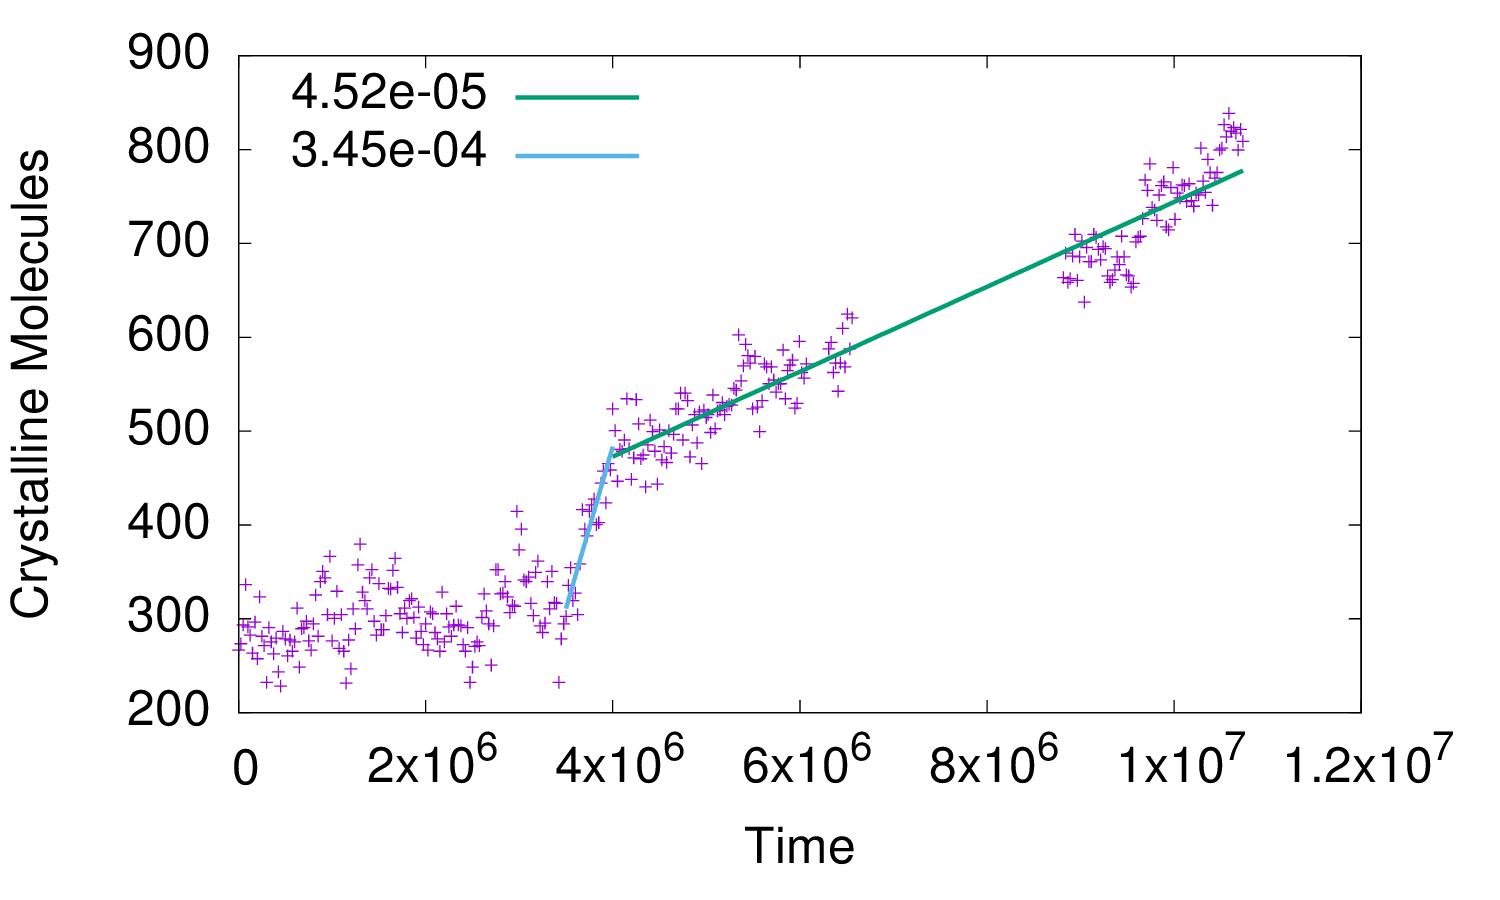
\includegraphics[width=0.5\textwidth]{done_crys_growth}
    \caption{Crystal growth of the \sone molecule. The region of growth can be fitted with a line of gradient \num{1.434e-8}.}
\end{figure}



\chapter{Conclusion}

The molecules we have studies in this thesis show a diverse range of dynamic and structural behaviour. The small changes we made to the shapes of our molecules made sufficient changes to their local structural rigidity that the dynamic properties of the liquid changed by orders of magnitude.

Along with changes to the local rigidity in the amorphous phase, the local structure of the ordered phase can be dramatically changed with small modifications to the shape. Small changes to the shape of a molecule can dramatically affect the ordering in the crystal phase, with certain structures, for example \dcon, preferentially forming an orientationally disordered crystal structure.

The slow crystalline growth of molecular systems can be attributed to the slow dynamics at the melting point. The additional entropy of the rotations stabilise the liquid phase such that the dynamics at the melting point are slow. This means that while the rate of crystallisation is slow, relative to the structural relaxation time crystal growth is fast.

\section{Future Work}

\begin{itemize}
    \item A more detailed investigation of the coupling between the rotational and translational motion and how they influence overall dynamics.
    \item Further investigation of the local structural rigidity of molecules and how molecular shape influences the rigidity. Identify the properties of a shape that most strongly influence the local rigidity and how we can tune the rigidity.
    \item Investigate how an orientationally disordered crystal like that formed by the \dcon molecule influences properties of a solid.
\end{itemize}


\begin{appendix}

\chapter{}

\section{Compact Packings}
\label{sec:compact}

A compact packing is an arrangement of disks such that for each neighbour $D_i$ of a central disk $D$, there exists two discs $D_{i+1}$ and $D_{i-1}$ neighbour both $D_i$ and $D$~\cite{heppes:03,kennedy:06}. These packings are the most efficient way to pack space. There are a number of binary compact packings~\figref{compact packing} suitable for patterning with molecules.
\begin{figure}[htb]
    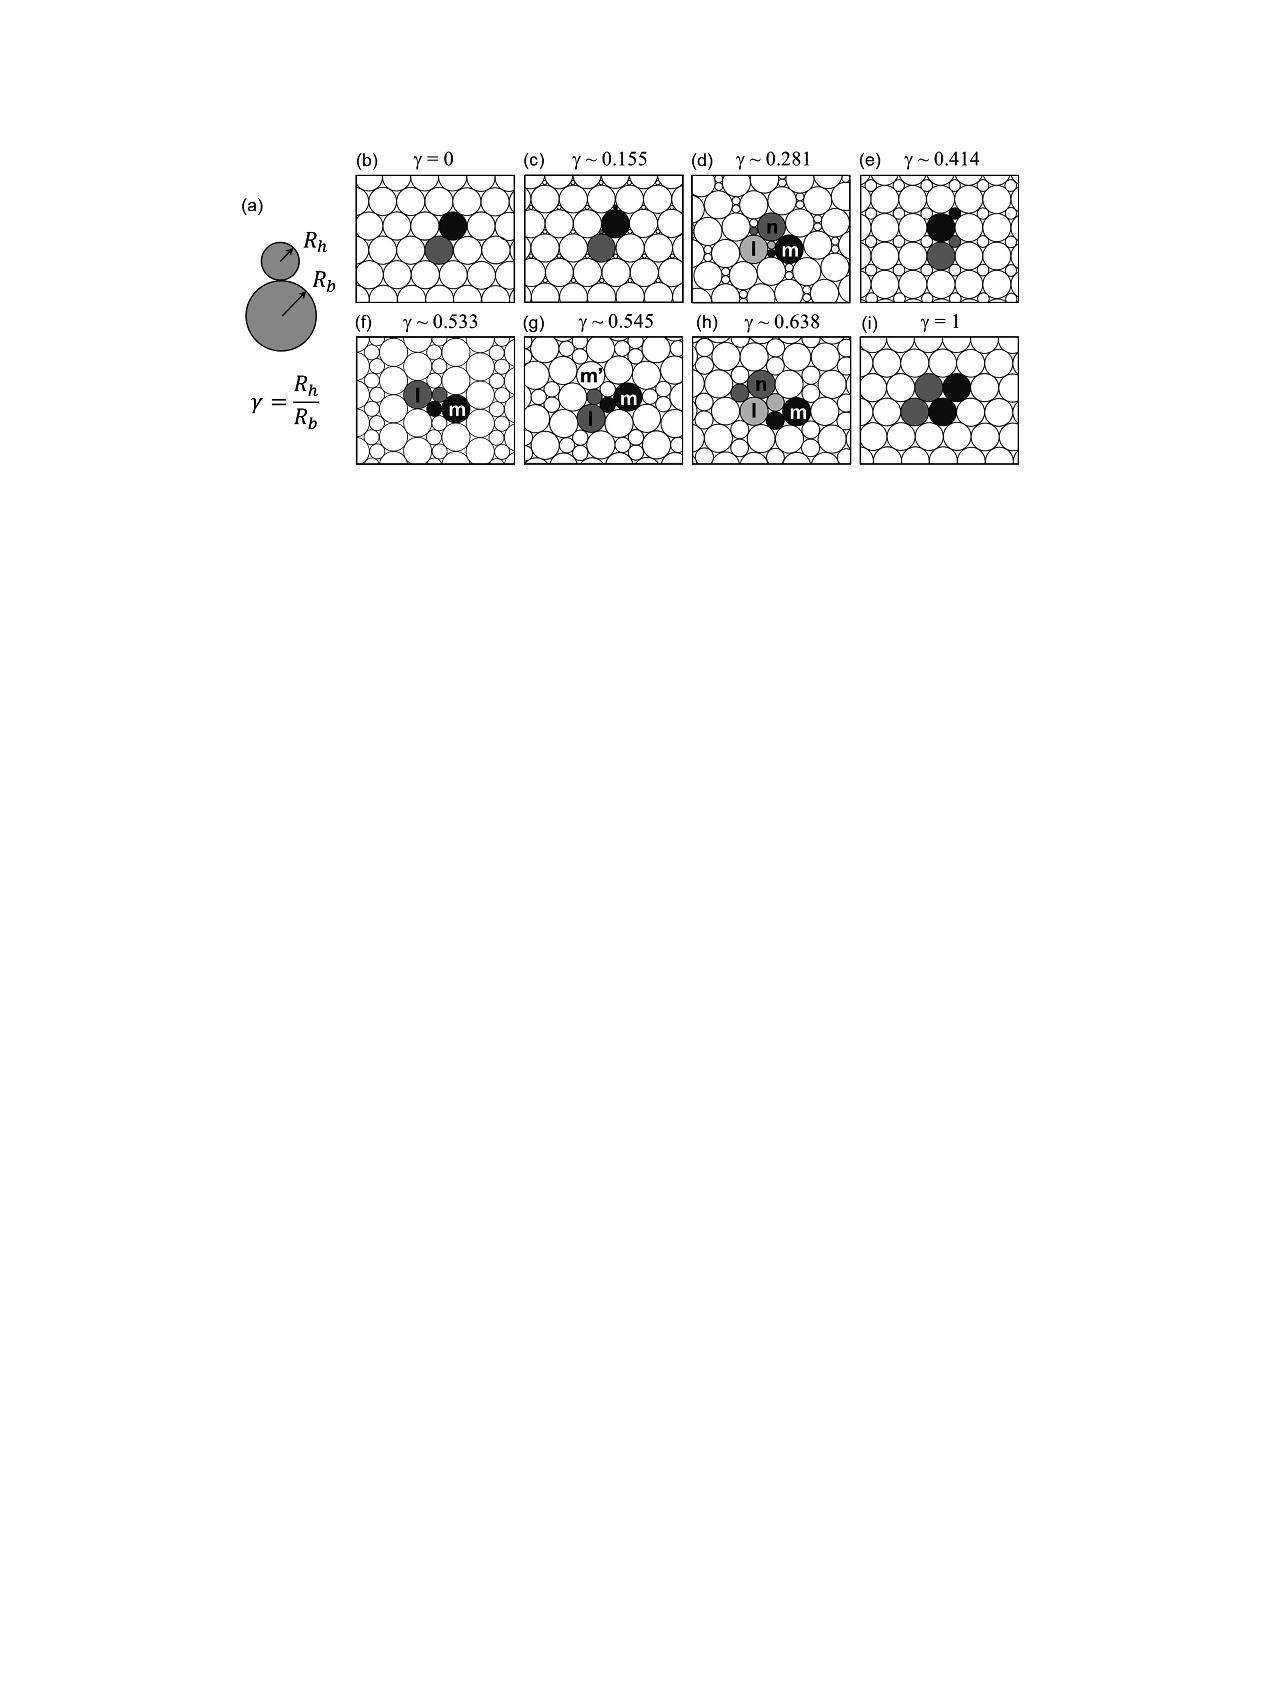
\includegraphics[width=\textwidth]{compact-packing}
    \caption{All the binary compact packings and allocations of molecules. The packing we are using in this thesis is (h).}
    \source{han:13}{American Physical Society}
    \label{fig:compact packing}
\end{figure}

\vspace{-3em}
\section{Wallpaper Groups}
\label{sec:wallpaper}

Wallpaper groups are a series of symmetry operations; rotations, mirror planes, and glide planes that describe the symmetry of a unit cell. There are 17 wallpaper groups in all and the low rotational symmetry wallpaper groups, including all wallpaper groups mentioned in this thesis are shown in \textfigref{wallpaper}
\begin{figure}[hbt]
    \centering
    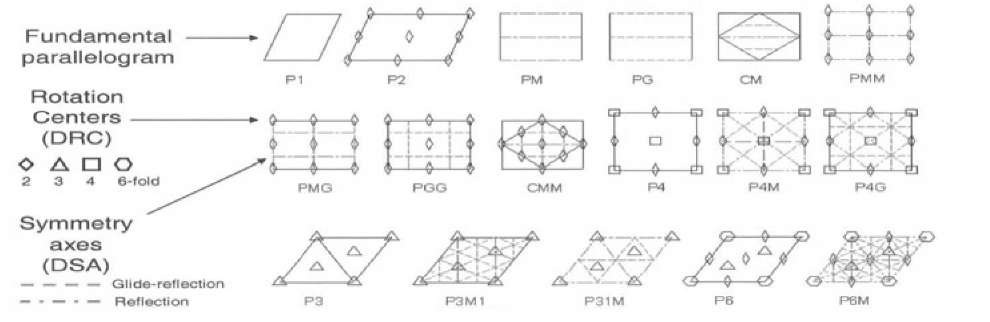
\includegraphics[width=\textwidth]{wallpaper_groups}
    \caption{The low rotational symmetry wallpaper groups showing the symmetry elements that comprise them.}
    \source[ccpd]{gagern:08}
    \label{fig:wallpaper}
\end{figure}
\end{appendix}


\printbibliography

\end{document}
